\chapter{Contexte / Environnement}
\label{chap:premierchapitre}

Dans ce chapitre, nous allons présenter l'entreprise dans laquelle j'ai travaillé, Sopra Steria, sa structure, l'agence 151 du secteur public, ainsi que le client auquel nos développement sont destinés : la Cnam.

\section{Sopra Steria}

Sopra Steria est né de la fusion en 2014 de deux des plus anciennes Entreprises de Services du Numérique françaises, Sopra et Steria, fondées respectivement en 1968 et 1969 et marquées toutes deux par un fort esprit entrepreneurial ainsi qu'un grand sens de l’engagement collectif au service de ses clients.

Le Groupe s'affirme comme un des leaders européens de la transformation numérique.

Suite à cette fusion le groupe compte près de 42 000 collaborateurs répartis dans plus de 20 pays et a réalisé un chiffre d’affaire de 3,8 milliards d’euros en 2017.

\begin{figure}[!h]
\centering

\includegraphics[width=0.8\textwidth]{images/chiffres_cles2017.jpg}
\caption{Sopra Steria : leader européen de la transformation numérique}
\end{figure}


Sopra Steria devient alors l'un des leader Européen de la transformation numérique.

\begin{figure}[!h]
\centering
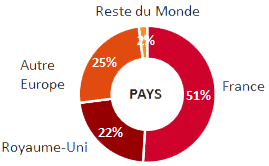
\includegraphics[width=0.5\textwidth]{images/payssoprasteria.png}
\caption{Sopra Steria : Répartition de l'activité en fonction des pays}
\end{figure}

Cette fusion a pris grâce à une forte complémentarité entre les deux entreprises : Sopra Group étant très implanté en France et peu à l'international, et Steria étant une entreprise reconnue à l'international, notamment en Europe.

//L’entreprise intervient dans de nombreux secteurs et domaines d’activité, et a du apprendre à faire face aux problèmes de managements intrinsèquement liés à sa taille et polyvalence.//

\begin{figure}[!h]
\centering
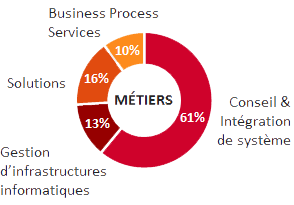
\includegraphics[width=0.5\textwidth]{images/metier_soprasteria.png}
\caption{Sopra Steria : Répartition des activités en fonction des métiers}
\end{figure}

Nous allons expliquer plus en détail les choix organisationnels de l’entreprise en prenant comme exemple notre secteur d’activité.

\section{Organisation du groupe}

//L'entreprise a choisi de diviser les secteurs d’activité et limiter le nombre d’échelons hiérarchiques au sein de chaque secteur, l’entreprise a également donné un grand pouvoir décisionnel et une grande indépendance aux collaborateurs exerçants des fonctions à responsabilités.//

La figure ci-dessous illustre la première division s’effectuant donc par secteur d’activité :

\begin{figure}[!h]
\centering
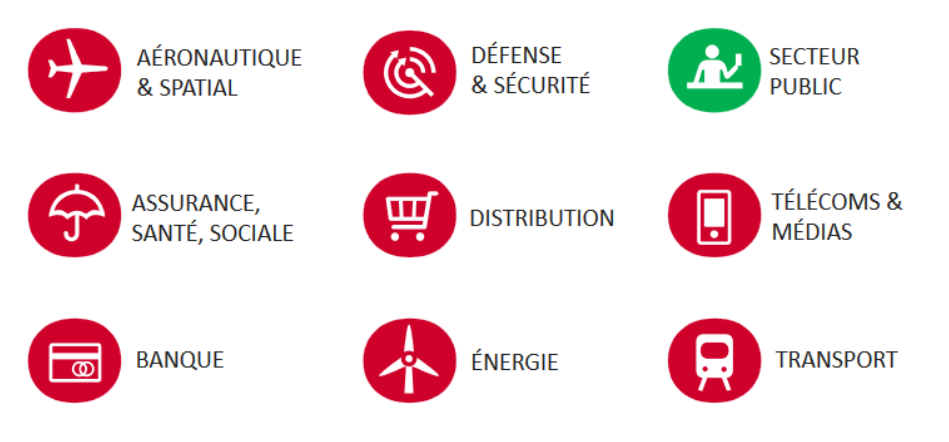
\includegraphics[width=0.8\textwidth]{images/secteurActivite.png}
\caption{Sopra Steria : Secteurs d'activités}
\end{figure}


Une Business Unit (BU) : Secteur public 
Le Secteur Public est le marché majoritaire chez Sopra Steria Group puisqu’il représente 25\% de son chiffre d’affaire.  La Business Unit du Secteur public est réparti sur 4 agences :  

\begin{itemize}
    \item Santé, Social, Emploi : Agence 151 (Sécurité sociale, Pole emploi, CNAMTS…), 
    \item echerche Enseignement : Agence 152 (ministère Éducation nationale, …), 
    \item dministration Centrale : Agence 156 (Mairie de Paris, DGFIP, ONP …), 
    \item onseil : Agence 155 (Clients transverses à toute la BU). Pour ma part, je travaille au sein de l’agence 151, pour le compte de la CNAM.
\end{itemize}


Au sein d'un même secteur d'activité, l'entreprise est divisée en agence qui fonctionnent comme des entreprises autonomes. Elles ont chacun un directeur d'agence, celui-ci dispose d'un grand pouvoir décisionnel au sein de son agence. Son objectif est que l'agence soit performante et fasse des bénéfices.
Une agence prend en charge de nombreux projets, dans notre cas, l'agence 151 gère les missions relevant du domaine de la Santé, du Social et de l’Emploi.
Ci-dessous la division au sein du secteur public.

\begin{figure}[!h]
\centering
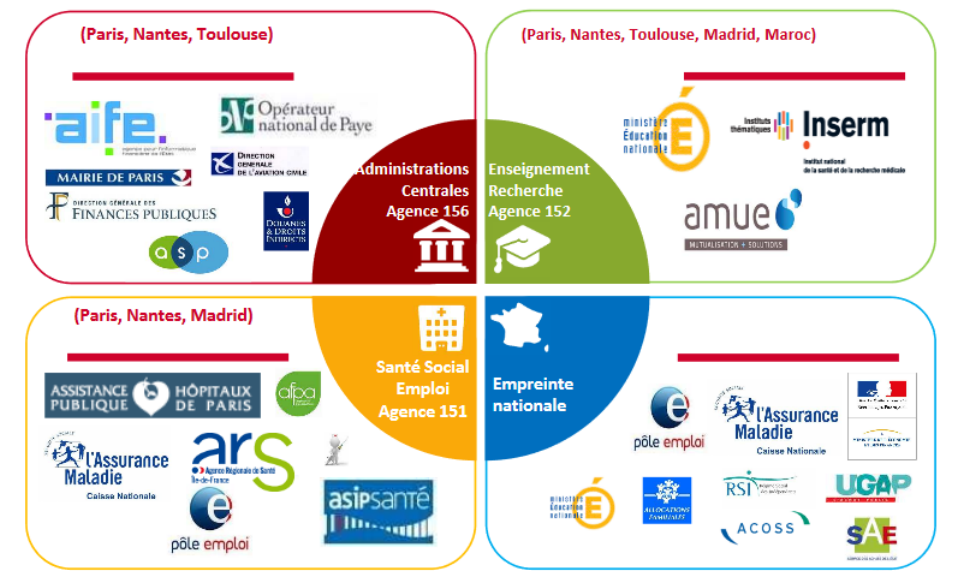
\includegraphics[width=1\textwidth]{images/divisionSecteurPublic.png}
\caption{Sopra Steria : Les agences du Secteur Public}
\end{figure}

\section{L'agence 151}

L'agence 151 est répartie dans plusieurs villes, soit dans les locaux de Sopra Steria, soit directement chez le client.

Les projets sont pris en charge par des équipes, et une équipe peut travailler sur plusieurs projets simultanément, de même plusieurs équipes peuvent travailler sur un même projet. Les équipes sont généralement d’une dizaine de membres, parmi lesquels on retrouve les rôles de :
- Chef de Projet (ou Project Manager),
- Analyste d’affaire (ou Business Analyst),
- Architecte,
- Expert produit (ou Product Expert),
- Solution Builder,
- Commercial.
Mon équipe est installée avec d'autres équipes Sopra Steria dont le client est la Cnam dans les locaux de Sopra Steria dans la tour Cytiscope à Montreuil. 

\section{Le client : la Cnam}

Chez Sopra Steria Group, plus de quatre cent collaborateurs travaillent pour le compte de la CNAM qui génère plus de 40 Millions d’euros de chiffre d’affaire. Ce chiffre est le plus important de toute la BU, ce qui fait de la CNAM un client d’importance maximale pour la société. Pour en dire un peu plus que la Caisse Nationale d’Assurance Maladie (CNAM), elle gère les branches maladie du régime général de la sécurité sociale, et représente :

\begin{itemize}
    \item 57 millions de bénéficiaires affiliés au régime général, 
    \item 4 assurés sur 5, 
    \item 75\% des dépenses de santé. 
\end{itemize}

Sopra Steria Group cherche à aider toutes ces entités en même temps dans leurs tâches quotidiennes. Les équipes de développement web (CNAMTS METIER) et de développement BI (CNAMTS BI) travaillent pour atteindre ces objectifs. Je suis moi même rattaché à la CNAM Métier. Ci-dessous la liste des projets/équipes de la CNAM Métier :

\begin{itemize}
    \item ARPEGE
    \item BIC : Briques I C
    \item CS Nantes
    \item DMP
    \item DPO
    \item DPRA
    \item INDIGO
    \item PPIL : Portail PILotage.
    \item OVERSI
\end{itemize}

\section{Le projet PPIL}
\subsubsection{Un Portail de PILotage}
PPIL permet d'assurer le suivi des projets de la CNAM.
Celui-ci répond à plusieurs besoins :
\begin{itemize}
    \item Centralisation : au sein d’un même espace des données de planification et de pilotage venant de Microsoft Project
    \item Suivi & Contrôle : vues consolidées facilitant le suivi et la vérification des données de pilotage (actualisation des données, cohérence, …)
    \item Évolutivité & Maintenance : socle permettant de mettre en place de nouvelles fonctionnalités et de les déployer pour tous les utilisateurs
    \item Communication : faciliter la diffusion de l’information
\end{itemize}
L'application PPIL a fait l'objet d'une refonte en 2017, désignée sous le nom PPIL V2. 

Les objectifs de cette version sont :
Prioritairement :
\begin{itemize}
    \item Les nouveautés concernant la gestion des projets
    \item Le fonctionnement de l’application PPIL V2 sur socle SharePoint 2013,
    \item L’iso-fonctionnalité par rapport à l’application PPIL V1, à l’exception de quelques fonctionnalités modifiées ou supprimées.
Secondairement :
    \item La simplification du portail,
    \item Des accès aux principales fonctionnalités dès la connexion en fonction des profils utilisateurs,
    \item Un usage simplifié et plus clair des fonctionnalités,
    \item La gestion des droits,
    \item La gestion des référentiels simples,
    \item La gestion des demandes et des lots.
\end{itemize}

Le Portail Pilotage est composé de différents Espaces dont l’accès est conditionné par le profil de l’utilisateur.
Les droits en lecture et/ou écriture selon le profil de l’utilisateur sont visibles dans le document de gouvernance (Gouvernance ci dessous).

Les utilisateurs accèdent à « Mon espace » et selon leurs profils, les informations restituées à l’écran varient. Les sous-espaces définis pour chaque profil suivent la description ci-après, dans l’ordre défini 

\subsubsection{Utilisateurs de PPIL :}
Opérationnel, comprenant les : 
\begin{itemize}
    \item Responsable DSI
    \item MOA
    \item Managers (Responsable de Direction ou Responsable de Département) 
    \item Chef de Projet
\end{itemize}
Stratégiques, comprenant les :
\begin{itemize}
    \item PMO
    \item Responsable de domaines
\end{itemize}

\subsubsection{Les acteurs et leurs niveaux d'autorisation}
\begin{figure}[!h]
\centering
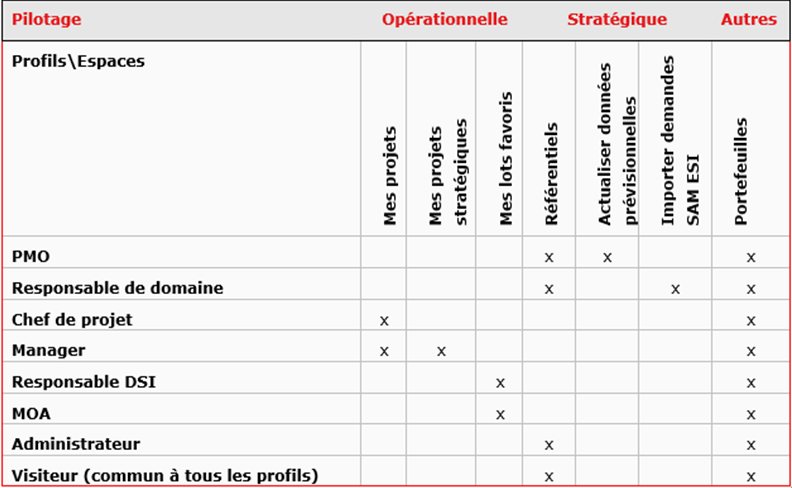
\includegraphics[width=0.8\textwidth]{images/ppil acteurs.png}
\caption{PPIL Les acteurs et leurs autorisations}
\end{figure}

\subsubsection{Lien LOT - Projet - PrtPalier}

(fig. \ref{fig:ppil lien lot projet prtpalier}).

\begin{figure}[!h]
\centering
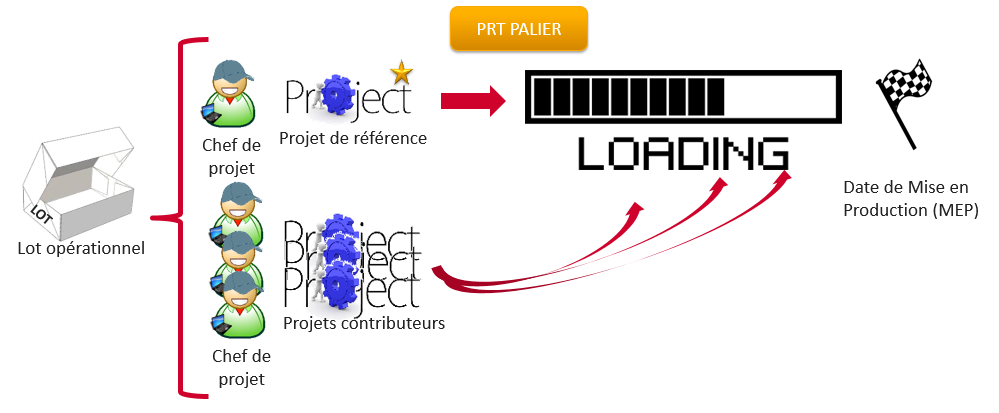
\includegraphics[width=1\textwidth]{images/ppil lien lot projet prtpalier.png}
\caption{PPIL lien lot projet PrtPalier}
\end{figure}

\subsubsection{Principe du Reporting - Suivi de projet}

AU sein de la CNAM, tous les acteurs d’un lot renseignent et mettent à jour le planning MSP de leur projet, en renseignant des données de type :
\begin{itemize}
    \item Avancement charges, 
    \item Dates des jalons, 
    \item consommé des ressources.
\end{itemize}

Les informations MSP sont remontées dans PPIL de plusieurs manières :
\begin{itemize}
    \item Batch 2 fois par jour
    \item Données prévisionnelles
    \item Actualiser les données MSP (CP) 
\end{itemize}

Tous les acteurs doivent renseigner les risques et problèmes rencontrés sur leur projet ainsi que l'état de leur projet (facultatif).

\subsubsection{Principe du Reporting - CP}
Le CP du projet référent doit soumettre le reporting du lot toutes les 2 semaines (météo, tendance, situation).

Une fois soumis le reporting du lot est visible par tous les utilisateurs du PPIL.

Le Manager doit saisir la note de conjoncture du lot tous les 2 mois : 
Cette action permet d'expliquer la situation opérationnelle du lot de manière moins technique, cette note de conjoncture est plus destiné aux supérieurs hiérarchiques ( Resp DSI).

\subsubsection{Chef de Projet}
Dashboard du CP :

\begin{itemize}
    \item Bulletin de santé
    \item Dérive des jalons
    \item Plan de charges équipe
    \item Accès à la liste de mes projets en cours
    \item Note de conjoncture à mettre à jour
    \item Alertes
    \item Rapports
\end{itemize}

Accès au portail PPIL via une délégation
Un délégant, a la possibilité de donner l’accès à ses espaces à un autre utilisateur délégataire.
Le délégataire choisit dans la liste des personnes dans le bandeau, sous le profil, le profil du délégant. Le délégataire possède tous les droits sur l’espace de son délégant.

\subsubsection{Visualiser des indicateurs}

PPIL permet aux différents profils d'utilisateurs de visualiser les indicateurs opérationnels sur son périmètre.

Par exemple, pour les profils CP, Manager, Responsable DSI et MOA, on peut visualiser :

\begin{itemize}
    \item l’indicateur Bulletin de santé
Les projets dont la tendance est en dégradation et/ou la météo est orageuse sont mis en évidence par cet indicateur.
Visualiser l’indicateur Dérive des jalons
Les projets dont le prochain jalon et/ou la date de mise en production est en dérive sont mis en évidence par cet indicateur.
    \begin{itemize}
        \item Un jalon est en dérive lorsqu’il existe une différence de plus de 7 jours entre les dates du dernier reporting et de celui fait il y a un mois.
    \end{itemize}
    \item 
\end{itemize}

Visualiser l’indicateur Avancement par phase : Chef de projet
    Les jalons de tous les projets aux états « En cours » du périmètre sont représentés dans cet indicateur.

Visualiser l’indicateur Plan de charge équipe : Manager
En cliquant sur le graphique, on accède au rapport du Capacity Planning

Visualiser l’indicateur Planning des MEP : Responsable DSI et MOA
Les lots dont la date de mise en production est comprise entre le mois passé et les six prochains mois sont placés sur une échelle de temps.

Accès au reporting
Dans les indicateurs dans lesquels sont affichés les noms des projets, en cliquant sur le nom d’un projet :
\begin{itemize}
    \item En tant que Manager, Responsable DSI et MOA, on accède à la restitution du reporting
    \item En tant que CP, on accède à la saisie du reporting
\end{itemize}
\subsubsection{Exécuter les actions rapides liées à mes projets}

Atteindre reporting et Actualiser les données MSP : Chef de projet

Visualiser le nombre de notes de conjoncture à mettre à jour : Manager


\subsubsection{Accéder à mes « informations opérationnelles » : CP, Manager, Responsable DSI et MOA}
Gérer les actions de mes projets : Chef de projet
Les actions remontées depuis une semaine ou moins sont taguées comme « Nouveau » et seules les actions dont la date d’échéance est soit dépassée, soit dont l’échéance est à venir sont affichées.
Consulter mes rapports opérationnels
En tant que CP, Manager, Responsable DSI et MOA, il est possible d’accéder au bloc « Rapports » dans « Mon espace » au niveau du sous-espace, situé dans la partie gauche de la page en dessous du bloc Alertes.
Visualiser la liste des projets / lots de mon périmètre


%%% Local Variables: 
%%% mode: latex
%%% TeX-master: "isae-report-template"
%%% End: 